
% ***************************************************
% Example of an internal chapter
% ***************************************************
%This is an internal chapter of the thesis.
%If you have a long title, you can supply an abbreviated version to print in the Table of Contents using the optional argument to the \chapter command.
\chapter[Literature review]{Literature review }
\label{Chap:label}	%CREATE YOUR OWN LABEL.
\pagestyle{headings}



Some of the concepts behind the proposed project, such as an Ethernet MAC or RISC-V processor are not new, there is a variety of previous works in these areas. This part of the proposal will explore the prior work related to the project. 




\section{Packet Filter Firewall}

Usually, the first line of defence against bad actors, it is firewalls play a vital component in computer networks and can become vastly complex. 
In essence, the job of a firewall is to isolate and restrict acess to an internal network from an external one \cite{BuildingInternetFirewalls}.

There are several types of Firewalls such as packet filters (PF), stateful packet firewalls and application firewalls \cite{FirewallsBook}. 
PFs are considered as stateless and traditionally filter exlcusively on the fields in the network (layer 2) and transport 
(layer 3) layer headers \cite{FirewallsBook}. Such fields include IP addresses, port numbers and protocol type.

Due to this, PFs are inherently simple and efficient. Consequently, they are widely available and can be either implemented in software or in 
hardware \cite{BuildingInternetFirewalls}. The book, \cite{BuildingInternetFirewalls}, also highlights some inherent flaws with PFs. These include not being able 
to suprress a sophisticated attacks and in some cases can be challenging to properly configure. More advanced firewalls can perform deep packet inspection and 
explore the contents of the higher layers to better evaluate a packets true intention \cite{FirewallsBook}. 




\section{Field Programmable Gate Arrays}
First introduced by Xilinx in 1984, field programmable gate arrays (FPGAs) allowed for large custom logic designs to be recognised without the need for 
expensive application specific integrated circuits (ASICs). More importantly, FPGAs did not suffer from the same scalability issues that
programmable array logic (PAL) encountered and has allowed for larger and more complex designs \cite{30YearsOfFPGA}. 

A big advantage to custom logic is the ability to create highly parallelised designs while also with a lower latency than software based serialised algorithms. 
As such, FPGAs became ubiquitous in both digital signal processing and for accelerating an assortment of computing architectures and processes \cite{FPGAComputing}.
System on chip (SoC) design with custom hardware acceleration modules is an active area research. As \cite{FPGAComputing} points out, there is a focus towards 
using both hardware and software in \textit{edge} devices due to growing numbers of IoT devices.

Several papers, \cite{LwIPFPGAFirewall} \cite{IPFPGAFirewall2000} \cite{packetFilteringFPGA}, have proposed a range of related FPGA based firewalls, all having 
slightly diffrent properties and using different classificiation mechanisms. Each of the propsoed firewalls in the afformentioned papers use custom hardware 
to first detect and then handle the incomming network packet. The key benefit to these firewalls is their high 
performance - namely, low latency, and high throughput. Article \cite{LwIPFPGAFirewall} proposed an ethernet firwall using LwIP and five-tuple binding 
to achieve a throughput of 950Mbps with a latency of 61.266us. A conference proceeding in 2000 \cite{IPFPGAFirewall2000} which used a comparator unit to check the 
fields of the IP header obtained a filtering rate of 500,000 packets per second. 

The enabling concept behind the above FPGA based firewalls is SoC design which involves integrating multiple components into a single package, or in this case a 
single FPGA. Often these will include small softcore microprocessors and some custom ethernet hardware like the proposed packet filters in \cite{LwIPFPGAFirewall}.
Softcore processors are configurable and can be modeled in a hardware description language (HDL) which can then be synthesised onto ASICs or FPGAs hardware 
\cite{SoftcoreBasedEmbeddedSystems}. Recently, the royalty free RISC-V based cores are a popular softcore architecture used on SoC design.


\section{RISC-V processor}
In the world of processor architectures, there are four major families, namely AMD64, x86, ARM and RISC-V. The two former instruction set architectures (ISA) 
are appart of the complex instructions sets (CISC) and are found in the majority of computers. ARM and RISC-V are a reduced version of the CISC family and 
subsequently fall under the RISC family and are ideal for low power microprocessors \cite{RV16Embedded}.

RISC-V is an open and royalty free ISA and as a result, a plethora of softcore based custom implementations have been designed \cite{CatalogRISCSoftcore}. 
Consequently, there is an abundance of articles dealving into RISC-V from evaluating the ISA \cite{InvestigatingRiscv} to creating multicore architectures
\cite{RiscVMulticore}. A 2019 paper, \cite{CatalogRISCSoftcore} evaluated a variety of different RISC-V softcore processors. RISC-V International have 
also published a list\footnote[1]{See: https://github.com/riscv/riscv-isa-manual/blob/master/marchid.md} of different RISC-V implementations 
that have a unique architecture ID. The majority of these are either written in a HDL for either application specific integrated circuits (ASICs) or FPGAs.
The \textit{NEORV32 RISC-V} softcore processor is written purely in vendor agnostic VHDL and importantly has a considerable amount of documentation. 

Being a softcore processor, control is given over which modules are implemented. Some basic features of the \textit{NEORV32 RISC-V} include 
UART, SPI, and GPIO interfaces \cite{neorv32Datasheet}. The datasheet, \cite{neorv32Datasheet}, also mentions that it supports a \textit{'Wishbone b4'} 
external bus interface. A Wishbone B4 (or just 'wishbone') interconnection is designed specifically to connect modular pieces of hardware together on a 
SoC into the memory mapped 32bit address space in the processor \cite{WishboneSpec}. This approach has the benefit of not neededing to create custom 
instructions for the microprocessor. 

\newpage

\section{Ethernet MAC}

First introduced in 1983, the IEEE 802.3 standard \cite{IEEE802.3-2012}, more commonly known by the name of 'Ethernet', defines the \textit{'Medium Access Control'} 
(MAC) protocol amongst other things for two or more devices to communicate over a network. This standard is just one part in the layered network 
models such as the OSI model or TCP/IP model, namely the network layer - layer 2. 

Several articles \cite{OptimisedEthernetMAC} \cite{EthernetAXI} \cite{EthernetRMII} about ethernet MACs implemented on FPGAs and 
intellectual property (IP) blocks can be found. One approach highlighted in \cite{OptimisedEthernetMAC} to creating a custom MAC is by using a finite state 
machine (FSM). 

Others have published both complete \footnote[1]{See: https://github.com/yol/ethernet\_mac} \footnote[2]{See: https://github.com/alexforencich/verilog-ethernet/} 
\footnote[3]{See: https://opencores.org/projects/ethernet\_tri\_mode} and uncomplete
\footnote[4]{See https://github.com/pabennett/ethernet\_mac} ethernet MACs for FPGAs as well.


A core function of the Ethernet MAC is to attach the required MAC layer headers to the head and tail of the layer 3 payload to create an ethernet packet.

\begin{figure}[h]
    \centering
    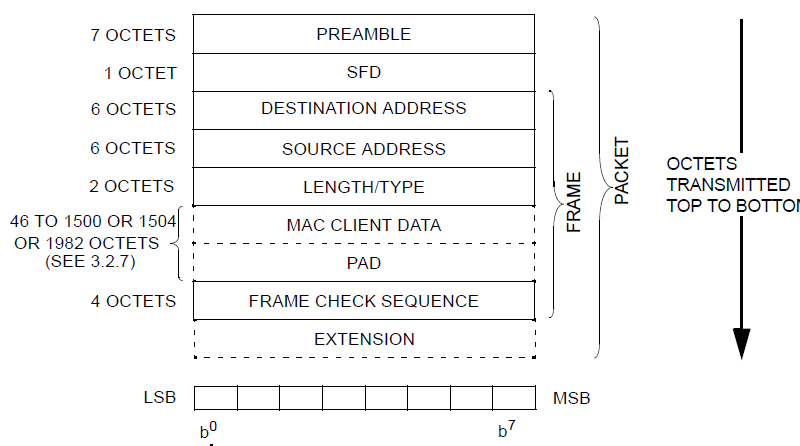
\includegraphics[width=0.65\textwidth]{Images/mac_packet.png}
    \caption{MAC layer headers \cite{IEEE802.3-2012}}
    \label{fig:vul}
\end{figure}


\section{Web servers and network stacks}
... The LwIP library is a popular lightweight TCP/IP stack which has been investigated in a plethora of research papers and projects. 


Recently, FreeRTOS have published their \textit{FreeRTOS-Plus-TCP} library which aims to provide ... over the LwIP stack. 






